\documentclass[]{article}

% Imported Packages
%------------------------------------------------------------------------------
\usepackage{amssymb}
\usepackage{amstext}
\usepackage{amsthm}
\usepackage{amsmath}
\usepackage{enumerate}
\usepackage{fancyhdr}
\usepackage[margin=1in]{geometry}
\usepackage{graphicx}
\usepackage{float}
%\usepackage{extarrows}
%\usepackage{setspace}
%------------------------------------------------------------------------------

% Header and Footer
%------------------------------------------------------------------------------
\pagestyle{plain}  
\renewcommand\headrulewidth{0.4pt}                                      
\renewcommand\footrulewidth{0.4pt}                                    
%------------------------------------------------------------------------------

% Title Details
%------------------------------------------------------------------------------
\title{Deliverable \#2 Template}
\author{SE 3A04: Software Design II -- Large System Design}
\date{}                               
%------------------------------------------------------------------------------

% Document
%------------------------------------------------------------------------------
\begin{document}

\maketitle	
\noindent{\bf Tutorial Number:} T01\\
{\bf Group Number:} G3 \\
{\bf Group Members:} 
\begin{itemize}
	\item List all Group Member Names (as listed in Avenue)
	\item You do not need to use student \#s or macid (keep those private).
\end{itemize}

\section*{IMPORTANT NOTES}
\begin{itemize}
	%	\item You do \underline{NOT} need to provide a text explanation of each diagram; the diagram should speak for itself
	\item Please document any non-standard notations that you may have used
	\begin{itemize}
		\item \emph{Rule of Thumb}: if you feel there is any doubt surrounding the meaning of your notations, document them
	\end{itemize}
	\item Some diagrams may be difficult to fit into one page
	\begin{itemize}
		\item Ensure that the text is readable when printed, or when viewed at 100\% on a regular laptop-sized screen.
		\item If you need to break a diagram onto multiple pages, please adopt a system of doing so and thoroughly explain how it can be reconnected from one page to the next; if you are unsure about this, please ask about it
	\end{itemize}
	\item Please submit the latest version of Deliverable 1 with Deliverable 2
	\begin{itemize}
		\item Indicate any changes you made.
	\end{itemize}
	\item If you do \underline{NOT} have a Division of Labour sheet, your deliverable will \underline{NOT} be marked
\end{itemize}

\newpage
\section{Introduction}
\label{sec:introduction}
% Begin Section

This high-level overview will describe the software architecture behind \textbf{GeoLens}, a community-driven application designed to identify locations using images, descriptions and discussions. This document outlines the design considerations behind the overall software architecture, and how its various subsystems interact.  

\subsection{Purpose}
\label{sub:purpose}
% Begin SubSection
This document serves as a technical guideline for the internal stakeholders of \textbf{GeoLens}, including project managers, developers, investors, and team members, ensuring a clear understanding of the system's overall structure and architecture. This document provides a high-level overview of the \textbf{GeoLens} system architecture, discussing the rationale behind the design considerations of the overall systems and its various subsystems. The SRS for \textbf{GeoLens} should be reviewed before reading this document as it contains essential technical information that will provide a better understanding of this document.% End SubSection

\subsection{System Description}
\label{sub:system_description}
% Begin SubSection
\textbf{GeoLens} follows a blackboard architectural style, a design which enables the multiple specialized AI models to collaboratively analyze and refine locations from user input. The blackboard architecture style supports the adaptability of AI models and is flexible to handle uncertainties in information. The subsystems of \textbf{GeoLens} follow a repository architectural style. The repository style was selected due to its ability to securely store, structure, and update information in such a manner that keeps the information consistent and allows for the easy retrieval of information. 

% End SubSection

\subsection{Overview}
\label{sub:overview}
% Begin SubSection
A breakdown of the document organization is below:
\begin{itemize}
  \item \textbf{Section 2}: An Analysis Class Diagram for \textbf{GeoLens}, outlining the system’s overall structure.
  \item \textbf{Section 3}: Discusses the architectural design of the system, elaborating on the design decisions behind the architecture and any considered design alternatives.
  \item \textbf{Section 4}: Discusses the classes of our system including their interactions and relationships through Class Responsibility Collaboration (CRC) Cards.
\end{itemize}

% End SubSection

% End Section

\section{Analysis Class Diagram}
\label{sec:analysis_class_diagram}
% Begin Section
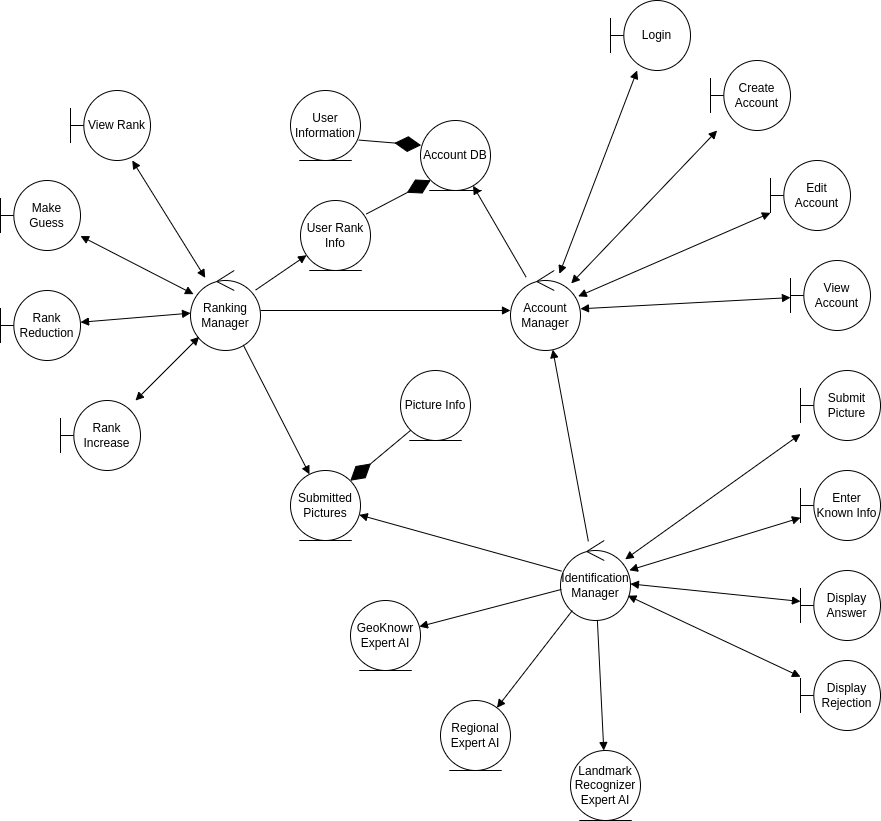
\includegraphics[scale=0.5]{analysis_class_diagram}
% End Section


\section{Architectural Design}
\label{sec:architectural_design}
% Begin Section
This section should provide an overview of the overall architectural design of your application. Your overall architecture should show the division of the system into subsystems with high cohesion and low coupling.

\subsection{System Architecture}
\label{sub:system_architecture}
% Begin SubSection


GeoLens uses Data-Centered Architecture, specifically the Blackboard Architecture. This style is commonly used for AI-driven and data-centric applications. In this architecture, multiple experts (knowledge sources) work collaboratively by contributing partial solutions to a shared data structure (the blackboard). The blackboard serves as a central repository, allowing various AI models to analyze and refine user-submitted images collaboratively. The Orchestrator (controller) manages this process by determining when a sufficient level of confidence has been reached before delivering a final result to the user. The system evolves dynamically as different subsystems process data and update the blackboard with new insights.\\

\noindent Within the system, several subsystems are defined as follows:\\

\renewcommand{\arraystretch}{1.3} % Adjust row height for better readability
\begin{table}[h]
    % \centering
    \begin{tabular}{|p{4cm}|p{7cm}|p{4cm}|} 
        \hline
        \textbf{Subsystem} & \textbf{Purpose} & \textbf{Architectural Style} \\
        \hline
        \textbf{Account Manager} & Manages user authentication, account creation, profile updates, and interactions with the account database. & 
        Repository Architecture \\
        \hline
        \textbf{Identification Manager} & Handles the image submission process, delegates analysis to AI experts, and processes identification results. & Blackboard Architecture \\
        \hline
        \textbf{Ranking Manager} & Manages user rankings based on accuracy, updates reputation scores, and retrieves ranking information. & Repository Architecture \\
        \hline
    \end{tabular}
\end{table}

\noindent Subsystem relationships are defined in section 3.2 of this document.\\

\noindent In addition, two databases are present in this architecture. A user database to keep track of user details, and a user ranking database to rank users on a leaderboard based on their identification results.\\

\noindent The Blackboard Architecture was selected because it allows for incremental problem-solving, parallel processing, and scalability. AI experts such as General Expert AI, Regional Expert AI, and Google Maps Landmark API work independently (asynchronously) and contribute partial solutions to the shared blackboard. This ensures that predictions are refined collaboratively without requiring direct interaction between AI models and that as fresh data becomes available, the blackboard updates each of its experts with the latest data. In this case, the data-store (blackboard) is active and the experts (knowledge sources) are passive, because the data-store controls the flow of logic. Unlike the Repository Architecture, where components interact with a passive data store, the Blackboard Architecture is event-driven, meaning that knowledge sources (AI models) react dynamically to changes in the blackboard. The Orchestrator manages the process of determining which expert to call on for information. This results in more adaptive and intelligent decision-making, making it well-suited for GeoLens’s AI-driven image analysis.\\

\noindent Additionally, structured data is managed using the Repository Architecture, namely for user account and ranking data. Because account actions include retrieval, updating, deletion, and insertion, this subsystem makes sense when it has access to a shared database. Software components in a pure data-centered architecture rely on a central data store rather than direct communication with one another. For systems like database management systems (DBMS), library information systems, and user authentication frameworks, where organized data consistency is really important, the repository architecture is perfect. The Repository Architecture guarantees data integrity, accessibility, and controlled alterations without needless complexity because account and ranking data depend on well-structured, transactional procedures rather than dynamic, event-driven problem-solving. \\

\begin{figure}[H]
    \centering
    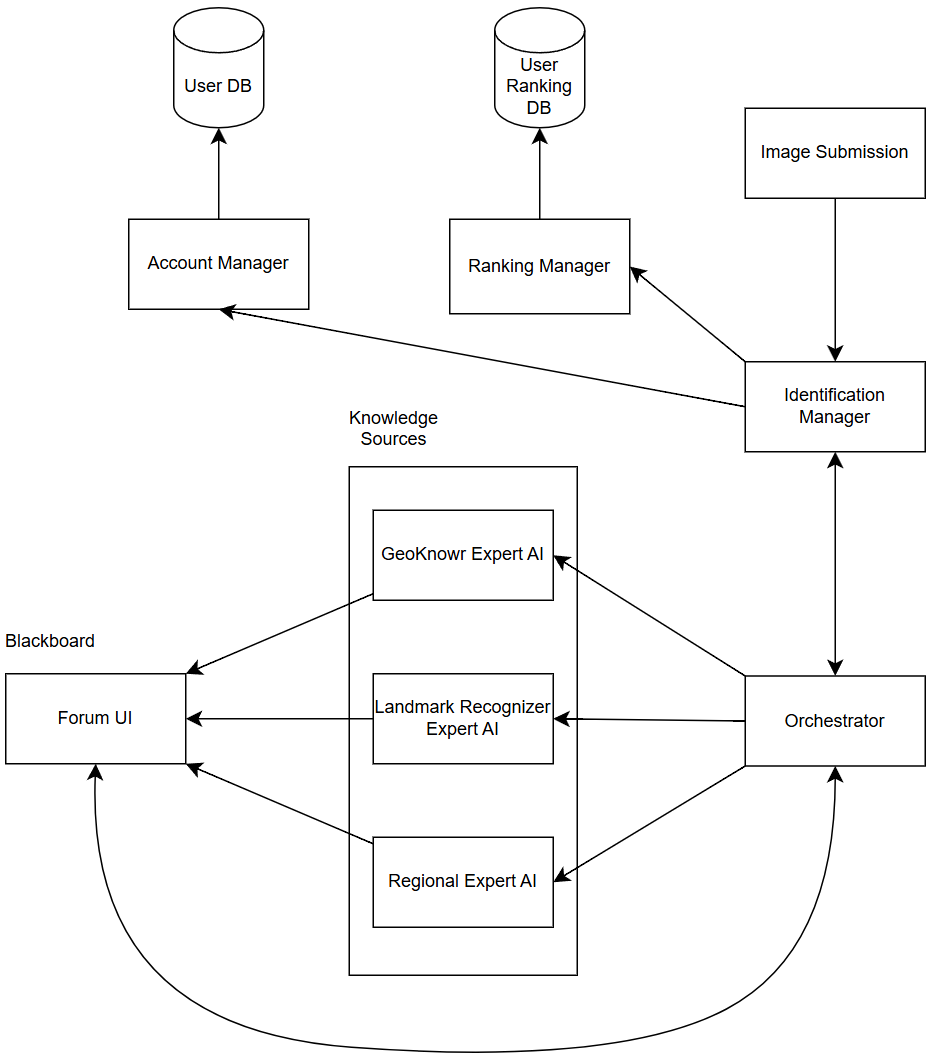
\includegraphics[width=1\linewidth]{system_architecture.png}
    \textbf{\caption{System Architecture}}
    \label{fig:system_architecture}
\end{figure}

\noindent Despite being considered, alternative architectural styles were not selected. The inability of Model-View-Controller (MVC) to have incremental problem-solving or collaboratively revise AI-generated solutions made it unsuitable for handling dynamic, AI-driven reasoning. The main goal of MVC is to structure user interaction, which helps to organize UI elements but doesn't help in asynchronous AI collaboration. Since GeoLens needs a system that allows several experts to iteratively improve predictions, Blackboard is a better option.\\

\noindent Pipe-and-Filter Architecture wasn't chosen either, because of its sequential processing approach, which prevents the flexible, real-time decision-making required for GeoLens. It is challenging to adapt AI processing dynamically in a Pipe-and-Filter system since input travel linearly through pipes and filters which is a synchronous process. Essentially, the next step cannot start until the current step has completed. The inflexible pipeline structure of Pipe-and-Filter would not allow for the necessary flexibility because multiple AI specialists would need to evaluate the same image concurrently and iteratively enhance the outcome.\\

\noindent Lastly, the Batch Sequential Architecture was also rejected because it is intended for processing data in discrete batches rather than real-time AI decision-making. Instantaneous picture analysis and response in GeoLens is incompatible with batch sequential systems, which process massive datasets at predetermined intervals. The Blackboard Architecture, on the other hand, allows for quicker and more accurate results by allowing experts to add insights as soon as they become available.\\

% End SubSection

\subsection{Subsystems}
\label{sub:subsystems}
% Begin SubSection
 \noindent Provide a list of your subsystems, with a brief description of each. Be sure to document its purpose and relationship to other subsystems.\\

 \noindent The Account Manager subsystem is responsible for all user-related actions, such as login, account creation, and profile modifications. It interacts with the User DB to securely store and retrieve user information. Since user data must be structured, persistent, and easily retrievable, the Repository Architecture is the most appropriate choice for this subsystem. \\

\noindent The Identification Manager subsystem oversees the image analysis process. When a user submits an image, this subsystem sends it to the Orchestrator (controller), which in turn sends it to multiple AI models (GeoKnowr Expert AI, Ladnmark Recognizer Expert AI, and Regional Expert API) for evaluation. Each AI component contributes its results to the Blackboard, where the Orchestrator refines predictions based on confidence scores. The Blackboard Architecture allows for collaboration among AI models, ensuring accurate and efficient identification. \\

\noindent The Ranking Manager subsystem tracks user rankings and reputation scores. When users submit guesses, their accuracy is assessed, and ranking adjustments are made accordingly. The Ranking Manager retrieves and updates user rankings from the User Ranking DB, ensuring that reputation data remains consistent. This subsystem follows the Repository Architecture, as ranking data needs to be stored persistently and accessed efficiently.
% End SubSection

% End Section
	
\section{Class Responsibility Collaboration (CRC) Cards}
\label{sec:class_responsibility_collaboration_crc_cards}
% Begin Section
This section should contain all of your CRC cards.

\begin{itemize}
	\item Provide a CRC Card for each identified class
	\item Please use the format outlined in tutorial, i.e.,
	\begin{table}[ht]
		\centering
		\begin{tabular}{|p{8cm}|p{8cm}|}
		\hline 
		 \multicolumn{2}{|l|}{\textbf{Class Name:} View Rank (Boundary)} \\
		\hline
		\textbf{Responsibility:} & \textbf{Collaborators:} \\
		\hline
		(insert text) & Ranking Manager \\
		(insert text) & \\
		\vspace{1in} & \\
		\hline
		\end{tabular}
	\end{table}

	\begin{table}
		\centering
		\begin{tabular}{|p{5cm}|p{5cm}|}
		\hline 
		 \multicolumn{2}{|l|}{\textbf{Class Name:} Make Guess (Boundary)} \\
		\hline
		\textbf{Responsibility:} & \textbf{Collaborators:} \\
		\hline
		(insert text) & Ranking Manager \\
		(insert text) & \\
		\vspace{1in} & \\
		\hline
		\end{tabular}
	\end{table}
	
	\begin{table}
		\centering
		\begin{tabular}{|p{5cm}|p{5cm}|}
		\hline 
		 \multicolumn{2}{|l|}{\textbf{Class Name:} Rank Reduction (Boundary)} \\
		\hline
		\textbf{Responsibility:} & \textbf{Collaborators:} \\
		\hline
		(insert text) & Ranking Manager \\
		(insert text) & \\
		\vspace{1in} & \\
		\hline
		\end{tabular}
	\end{table}

	\begin{table}
		\centering
		\begin{tabular}{|p{5cm}|p{5cm}|}
		\hline 
		 \multicolumn{2}{|l|}{\textbf{Class Name:} Rank Increase (Boundary)} \\
		\hline
		\textbf{Responsibility:} & \textbf{Collaborators:} \\
		\hline
		(insert text) & Ranking Manager \\
		(insert text) & \\
		\vspace{1in} & \\
		\hline
		\end{tabular}
	\end{table}

	\begin{table}
		\centering
		\begin{tabular}{|p{5cm}|p{5cm}|}
		\hline 
		 \multicolumn{2}{|l|}{\textbf{Class Name:} Ranking Manager (Control)} \\
		\hline
		\textbf{Responsibility:} & \textbf{Collaborators:} \\
		\hline
		(insert text) & View Rank \\
		(insert text) & View Rank \\
		(insert text) & View Rank \\
		(insert text) & View Rank \\
		(insert text) & User Rank Info \\
		(insert text) & Submitted Pictures \\
		(insert text) & \\
		\vspace{1in} & \\
		\hline
		\end{tabular}
	\end{table}

	\begin{table}
		\centering
		\begin{tabular}{|p{5cm}|p{5cm}|}
		\hline 
		 \multicolumn{2}{|l|}{\textbf{Class Name:} User Information (Entity)} \\
		\hline
		\textbf{Responsibility:} & \textbf{Collaborators:} \\
		\hline
		(insert text) & Account DB \\
		(insert text) & \\
		\vspace{1in} & \\
		\hline
		\end{tabular}
	\end{table}

	\begin{table}
		\centering
		\begin{tabular}{|p{5cm}|p{5cm}|}
		\hline 
		 \multicolumn{2}{|l|}{\textbf{Class Name:} User Rank Info (Entity)} \\
		\hline
		\textbf{Responsibility:} & \textbf{Collaborators:} \\
		\hline
		(insert text) & Ranking Manager \\
		(insert text) & Account DB \\
		(insert text) & \\
		\vspace{1in} & \\
		\hline
		\end{tabular}
	\end{table}

	\begin{table}
		\centering
		\begin{tabular}{|p{5cm}|p{5cm}|}
		\hline 
		 \multicolumn{2}{|l|}{\textbf{Class Name:} Submitted Pictures (Entity)} \\
		\hline
		\textbf{Responsibility:} & \textbf{Collaborators:} \\
		\hline
		(insert text) & Ranking Manager \\
		(insert text) & Picture Info \\
		(insert text) & Identification Manager \\
		(insert text) & \\
		\vspace{1in} & \\
		\hline
		\end{tabular}
	\end{table}

	% Split here

	\begin{table}
		\centering
		\begin{tabular}{|p{5cm}|p{5cm}|}
		\hline 
		 \multicolumn{2}{|l|}{\textbf{Class Name:} Account Database)} \\
		\hline
		\textbf{Responsibility:} & \textbf{Collaborators:} \\
		\hline
		\vspace{1in} & \\
		\hline
		\end{tabular}
	\end{table}

	\begin{table}
		\centering
		\begin{tabular}{|p{5cm}|p{5cm}|}
		\hline 
		 \multicolumn{2}{|l|}{\textbf{Class Name:} Picture Info} \\
		\hline
		\textbf{Responsibility:} & \textbf{Collaborators:} \\
		\hline
		\vspace{1in} & \\
		\hline
		\end{tabular}
	\end{table}

	\begin{table}
		\centering
		\begin{tabular}{|p{5cm}|p{5cm}|}
		\hline 
		 \multicolumn{2}{|l|}{\textbf{Class Name:} Account Manager} \\
		\hline
		\textbf{Responsibility:} & \textbf{Collaborators:} \\
		\hline
		\vspace{1in} & \\
		\hline
		\end{tabular}
	\end{table}

	\begin{table}
		\centering
		\begin{tabular}{|p{5cm}|p{5cm}|}
		\hline 
		 \multicolumn{2}{|l|}{\textbf{Class Name:} Identification Manager} \\
		\hline
		\textbf{Responsibility:} & \textbf{Collaborators:} \\
		\hline
		\vspace{1in} & \\
		\hline
		\end{tabular}
	\end{table}

	\begin{table}
		\centering
		\begin{tabular}{|p{5cm}|p{5cm}|}
		\hline 
		 \multicolumn{2}{|l|}{\textbf{Class Name:} General Expert AI} \\
		\hline
		\textbf{Responsibility:} & \textbf{Collaborators:} \\
		\hline
		\vspace{1in} & \\
		\hline
		\end{tabular}
	\end{table}

	\begin{table}
		\centering
		\begin{tabular}{|p{5cm}|p{5cm}|}
		\hline 
		 \multicolumn{2}{|l|}{\textbf{Class Name:} Regional Expert AI} \\
		\hline
		\textbf{Responsibility:} & \textbf{Collaborators:} \\
		\hline
		\vspace{1in} & \\
		\hline
		\end{tabular}
	\end{table}

	\begin{table}
		\centering
		\begin{tabular}{|p{5cm}|p{5cm}|}
		\hline 
		 \multicolumn{2}{|l|}{\textbf{Class Name:} Google Maps Landmark API} \\
		\hline
		\textbf{Responsibility:} & \textbf{Collaborators:} \\
		\hline
		\vspace{1in} & \\
		\hline
		\end{tabular}
	\end{table}

	\begin{table}
		\centering
		\begin{tabular}{|p{5cm}|p{5cm}|}
		\hline 
		 \multicolumn{2}{|l|}{\textbf{Class Name:} Login} \\
		\hline
		\textbf{Responsibility:} & \textbf{Collaborators:} \\
		\hline
		\vspace{1in} & \\
		\hline
		\end{tabular}
	\end{table}

	\begin{table}
		\centering
		\begin{tabular}{|p{5cm}|p{5cm}|}
		\hline 
		 \multicolumn{2}{|l|}{\textbf{Class Name:} Create Account} \\
		\hline
		\textbf{Responsibility:} & \textbf{Collaborators:} \\
		\hline
		\vspace{1in} & \\
		\hline
		\end{tabular}
	\end{table}

	\begin{table}
		\centering
		\begin{tabular}{|p{5cm}|p{5cm}|}
		\hline 
		 \multicolumn{2}{|l|}{\textbf{Class Name:} Edit Account} \\
		\hline
		\textbf{Responsibility:} & \textbf{Collaborators:} \\
		\hline
		\vspace{1in} & \\
		\hline
		\end{tabular}
	\end{table}

	\begin{table}
		\centering
		\begin{tabular}{|p{5cm}|p{5cm}|}
		\hline 
		 \multicolumn{2}{|l|}{\textbf{Class Name:} View Account} \\
		\hline
		\textbf{Responsibility:} & \textbf{Collaborators:} \\
		\hline
		\vspace{1in} & \\
		\hline
		\end{tabular}
	\end{table}

	\begin{table}
		\centering
		\begin{tabular}{|p{5cm}|p{5cm}|}
		\hline 
		 \multicolumn{2}{|l|}{\textbf{Class Name:} Submit Picture} \\
		\hline
		\textbf{Responsibility:} & \textbf{Collaborators:} \\
		\hline
		\vspace{1in} & \\
		\hline
		\end{tabular}
	\end{table}

	\begin{table}
		\centering
		\begin{tabular}{|p{5cm}|p{5cm}|}
		\hline 
		 \multicolumn{2}{|l|}{\textbf{Class Name:} Enter Known Info} \\
		\hline
		\textbf{Responsibility:} & \textbf{Collaborators:} \\
		\hline
		\vspace{1in} & \\
		\hline
		\end{tabular}
	\end{table}

	\begin{table}
		\centering
		\begin{tabular}{|p{5cm}|p{5cm}|}
		\hline 
		 \multicolumn{2}{|l|}{\textbf{Class Name:} Display Answer} \\
		\hline
		\textbf{Responsibility:} & \textbf{Collaborators:} \\
		\hline
		\vspace{1in} & \\
		\hline
		\end{tabular}
	\end{table}

	\begin{table}
		\centering
		\begin{tabular}{|p{5cm}|p{5cm}|}
		\hline 
		 \multicolumn{2}{|l|}{\textbf{Class Name:} Display Rejection} \\
		\hline
		\textbf{Responsibility:} & \textbf{Collaborators:} \\
		\hline
		\vspace{1in} & \\
		\hline
		\end{tabular}
	\end{table}

\end{itemize}
% End Section

\appendix
\section{Division of Labour}
\label{sec:division_of_labour}
% Begin Section
\textbf{Nesbitt, Matthew:}
\begin{itemize}
	\item 2.3 User Characteristics
	\item 2.4 Constraints
	\item 2.5 Assumptions and Dependencies
	\item 2.6 Apportioning of Requirements
	\item 3 Use Case Diagram
	\item Brainstormed creative idea as group:
		\subitem - Gamified guessing system.
\end{itemize}

\includegraphics[scale=0.15]{mattsignature.jpg}

\textbf{Klisuric, Petar:}
\begin{itemize}
	\item 5.5 Maintainability and Support Requirements
	\item 5.6 Security Requirements
	\item 5.7 Cultural and Political Requirements
	\item 5.8 Legal Requirements
	\item 1.4 References
    \item Brainstormed creative idea as group:
		\subitem - Leaderboard within the gamified guessing system.
\end{itemize}
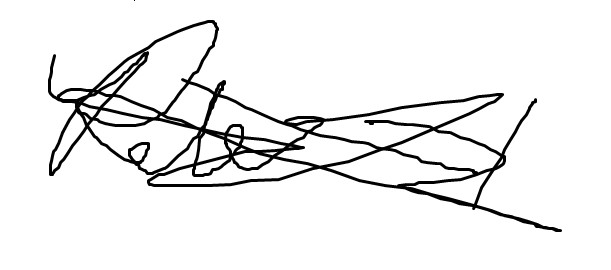
\includegraphics[scale=0.15]{petarsignature.jpg}

\textbf{Rooprai, Mankaran:}
\begin{itemize}
	\item 3.1 System Architecture
	\item 3.2 Subsystems
	\item Figure 2. System Architecture
	\item Created subsytems table in section 3.1
\end{itemize}

\includegraphics[scale=0.15]{mankaransignature.png}

\textbf{Nielsen, Claire}
\begin{itemize}
        \item 4 Highlights of Functional Requirements
            \subitem - Main Business Events
            \subitem - Viewpoints
            \subitem - Interpretation
\end{itemize}

\includegraphics[scale=0.15]{clairesignature.jpg}

\textbf{Bornomala, Anindita}
\begin{itemize}
        \item 5 Non-Functional Requirements
            \subitem - Look and Feel Requirements (5.1)
            \subitem - Usability and Humanity Requirements (5.2)
            \subitem - Performance Requirements (5.3)
            \subitem - Operational and Environmental Requirements (5.4)
            \subitem - References (1.4)
\end{itemize}

\includegraphics[scale=0.50]{bornosignature.png}

\textbf{Lam, Robert}
\begin{itemize}
        \item Introduction
        \item 1.1 Purpose
        \item 1.2 Scope
        \item 1.3 Definitions and Acronyms
        \item Brainstormed experts as a group:
		    \subitem - \textbf{GeoKnowr} AI.
\end{itemize}

\includegraphics[scale=1]{robertsignature.png}
% Begin Section
Include a Division of Labour sheet which indicates the contributions of each team member. This sheet must be signed by all team members.
% End Section


\end{document}
%------------------------------------------------------------------------------
